\documentclass[tikz]{standalone}
\usetikzlibrary{chains,shadows.blur}
% For decorating a path with text.
\begin{document}
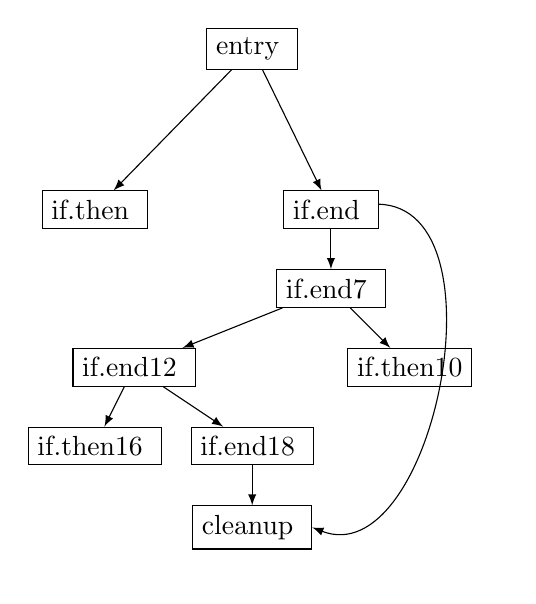
\begin{tikzpicture}[node distance = 8mm, start chain = going below, box/.style = {draw,rounded corners, on chain, align=center}]
\node[box, sharp corners] (entry) at (2, -1.00) { entry };
\node[box, sharp corners] (if_then) at (0.0, -2.00) { if.then };
\node[box, sharp corners] (if_end) at (3.0, -2.00) { if.end };
\node[box, sharp corners] (if_end7) at (3.0, -3.00) { if.end7 };
\node[box, sharp corners] (if_then10) at (4.0, -4.00) { if.then10};
\node[box, sharp corners] (if_end12) at (.5, -4.00) { if.end12 };
\node[box, sharp corners] (if_then16) at (0.0, -5.00) { if.then16 };
\node[box, sharp corners] (if_end18) at (2, -5.00) { if.end18 };
\node[box, sharp corners] (cleanup) at (2, -6.00) { cleanup };

\begin{scope}[rounded corners,-latex]
\path [color=black] (entry) edge[ bend left=0 ] (if_end);
\path [color=black] (entry) edge[ bend left=0 ] (if_then);
\path [color=black] (if_end) edge[ bend left=0 ] (if_end7);
\path [color=black] (if_end) edge[ bend left=100 ] (cleanup.east);
\path [color=black] (if_end7) edge[ bend left=0 ] (if_end12);
\path [color=black] (if_end7) edge[ bend left=0 ] (if_then10);
\path [color=black] (if_end12) edge[ bend left=0 ] (if_end18);
\path [color=black] (if_end12) edge[ bend left=0 ] (if_then16);
\path [color=black] (if_end18) edge[ bend left=0 ] (cleanup);
\end{scope}
\end{tikzpicture}

\end{document}

